\documentclass[11pt,letterpaper]{article}
\pdfoutput=1
\usepackage{jheppub}

\usepackage[utf8]{inputenc}

\usepackage{color}
\usepackage{graphicx}
\usepackage{tabularx}
\usepackage{xspace}

\usepackage{verbatim}
\usepackage{amsmath}
\usepackage{amssymb}
\usepackage[caption=false]{subfig}
\usepackage{url}
\usepackage{bbold}
\usepackage{slashed}
\usepackage{array}

\usepackage{multirow}
\usepackage{threeparttable}
\usepackage{paralist}

\newcommand{\GeV}{\text{GeV}}
\newcommand{\TeV}{\text{TeV}}
\newcommand{\SO}{\text{SO}}
\newcommand{\SU}{\text{SU}}
\newcommand{\SM}{\text{SM}}

\newcommand{\U}{\text{U}}
\newcommand{\CKM}{\text{CKM}}
\newcommand{\eff}{\text{eff}}

\newcommand{\genang}[2]{{\lambda^{#1}_{#2}}}


\newcommand{\ev}{\text{event}}
\newcommand{\jet}{\text{jet}}
\newcommand{\jets}{\text{jets}}
\newcommand{\subj}{\text{subjet}}
\newcommand{\subjs}{\text{subjets}}
\newcommand{\cut}{\text{cut}}
\newcommand{\trim}{\text{trim}}
\newcommand{\Ecut}{E_{{\rm cut}}}

\newcommand{\ptc}{p_{T{\rm cut}}}
\newcommand{\ptsubc}{p_{T{\rm subcut}}}

\newcommand{\sub}{\text{sub}}
\newcommand{\miss}{\text{miss}}

\newcommand{\pythia}{\textsc{Pythia~8}\xspace}
\newcommand{\herwig}{\textsc{Herwig++}\xspace}
\newcommand{\eventtwo}{\textsc{Event2}\xspace}
\newcommand{\vincia}{\textsc{Vincia}\xspace}
\newcommand{\sherpa}{\textsc{Sherpa}\xspace}

\newcommand{\FastJet}{\textsc{FastJet}\xspace}
\newcommand{\MadGraph}{\textsc{MadGraph}\xspace}

\newcommand{\df}{\text{d}}
\newcommand{\vev}[1]{\langle #1 \rangle}


\DeclareRobustCommand{\Sec}[1]{Sec.~\ref{#1}}
\DeclareRobustCommand{\Secs}[2]{Secs.~\ref{#1} and \ref{#2}}
\DeclareRobustCommand{\Secss}[3]{Secs.~\ref{#1}, \ref{#2}, and \ref{#3}}
\DeclareRobustCommand{\App}[1]{App.~\ref{#1}}
\DeclareRobustCommand{\Tab}[1]{Table~\ref{#1}}
\DeclareRobustCommand{\Tabs}[2]{Tables~\ref{#1} and \ref{#2}}
\DeclareRobustCommand{\Fig}[1]{Fig.~\ref{#1}}
\DeclareRobustCommand{\Figs}[2]{Figs.~\ref{#1} and \ref{#2}}
\DeclareRobustCommand{\Figss}[3]{Figs.~\ref{#1}, \ref{#2}, and \ref{#3}}
\DeclareRobustCommand{\Eq}[1]{Eq.~(\ref{#1})}
\DeclareRobustCommand{\Eqs}[2]{Eqs.~(\ref{#1}) and (\ref{#2})}
\DeclareRobustCommand{\Eqss}[3]{Eqs.~(\ref{#1}), (\ref{#2}), and (\ref{#3})}
\DeclareRobustCommand{\Ref}[1]{Ref.~\cite{#1}}
\DeclareRobustCommand{\Refs}[1]{Refs.~\cite{#1}}

\newcommand{\be}{\begin{equation}}
\newcommand{\ee}{\end{equation}}
\newcommand{\nn}{\nonumber}

\renewcommand{\textfraction}{0.10}
\renewcommand{\topfraction}{0.90}
\renewcommand{\bottomfraction}{0.90}
\renewcommand{\floatpagefraction}{0.65}

%% Reference commands %%
\newcommand{\mb}[1]{\boldsymbol{#1}}
\newcommand{\bm}[1]{\boldsymbol{#1}}
\newcommand{\mbo}[1]{\boldsymbol{\overline{#1}}}

\usepackage{xspace}


\def\Tr{\mathop{\rm Tr}}
\newcommand{\rep}[1]{\mathbf{#1}}
\newcommand{\conjrep}[1]{\overline{\mathbf{#1}}}


\renewcommand{\a}{\alpha}
\renewcommand{\b}{\beta}
\newcommand{\e}{\epsilon}
\newcommand{\D}{\Delta}
\renewcommand{\l}{\lambda}
\renewcommand{\th}{\theta}
\newcommand{\bq}{\bar{q}}
\newcommand{\zcut}{z_{\rm cut}}

\newcommand{\IZ}{\mathbb{Z}}
\newcommand{\cD}{\mathcal{D}}
\newcommand{\cL}{\mathcal{L}}
\newcommand{\cR}{\mathcal{R}}
\newcommand{\cF}{\mathcal{F}}
\newcommand{\cI}{\mathcal{I}}
\newcommand{\cK}{\mathcal{K}}
\newcommand{\beq}{\begin{eqnarray}}
\newcommand{\eeq}{\end{eqnarray}}

\newcommand{\F}{\mathcal{F}}
\newcommand{\Ft}{\widetilde{\mathcal{F}}}
\newcommand{\G}{\mathcal{G}}
\newcommand{\Gt}{\widetilde{\mathcal{G}}}
\newcommand{\HH}{\mathcal{H}}
\newcommand{\HHt}{\widetilde{\mathcal{H}}}
\newcommand{\ord}[1]{\mathcal{O}\!\left(#1\right)}

\newcommand*\numcircledmod[1]{#1 \!\!\! \bigcirc}

\newcommand{\Njet}{\widetilde{N}_{\rm jet}}
\newcommand{\dN}[1]{\Delta_{#1}}
\newcommand{\dNpm}{\Delta_{2\pm}}
\newcommand{\dNp}{\Delta_{2+}}
\newcommand{\dNm}{\Delta_{2-}}
\newcommand{\dNtm}{\Delta_{3-}}

\newcommand{\cT}{\mathcal{T}}
\newcommand{\as}{\alpha_s}
\renewcommand{\angle}{\theta}


\newcommand{\ecf}[2]{e_{#1}^{(#2)}} 
\newcommand{\ecfnobeta}[1]{e_{#1}} 

\newcommand{\ecfvar}[3]{{_{#1}e_{#2}^{(#3)}}} 
\newcommand{\ecfvarnobeta}[2]{{_{#1}e_{#2}}} 

\newcommand{\Dobs}[2]{D_{#1}^{(#2)}} 
\newcommand{\Dobsnobeta}[1]{D_{#1}} 

\newcommand{\Xobs}[2]{X_{#1}^{(#2)}} 

\newcommand{\Cobs}[2]{C_{#1}^{(#2)}} 
\newcommand{\Cobsnobeta}[1]{C_{#1}} 

\newcommand{\Nsub}[2]{\tau_{#1}^{(#2)}}
\newcommand{\Nsubnobeta}[1]{\tau_{#1}}


%\newcommand{\pythia}[1]{\textsc{Pythia\xspace #1}}
\newcommand{\madgraph}[1]{\textsc{MadGraph5\xspace #1}}
\newcommand{\fastjet}[1]{\textsc{FastJet\xspace #1}}
%\newcommand{\herwig}[1]{\textsc{Herwig\xspace #1}}
\newcommand{\herwigpp}[1]{\textsc{Herwig++\xspace #1}}
%\newcommand{\vincia}[1]{\textsc{Vincia\xspace #1}}
\newcommand{\nlojet}{\textsc{NLOJet++}}
%\newcommand{\sherpa}{\textsc{Sherpa}}
\newcommand{\ariadne}{\textsc{Ariadne}}
\newcommand{\geneva}{\textsc{Geneva}}
\newcommand{\dire}{\textsc{Dire}}




%\definecolor{darkgreen}{rgb}{0,0.5,0}
%\newcommand{\jdt}[1]{\textbf{\textcolor{darkgreen}{(#1 --jdt)}}}

%\definecolor{darkblue}{rgb}{0,0,0.5}
%\newcommand{\gs}[1]{\textbf{\textcolor{darkblue}{(#1 --gs)}}}

\definecolor{llblue}{rgb}{0,0.5,1.0}
\newcommand{\ijm}[1]{\textbf{\textcolor{llblue}{(#1 --ijm)}}}







\begin{document}


\title{Performance versus Robustness for Two-Prong Jet Substructure}

\author[a]{Disha Bhatia,}
\author[a]{Reina Camacho,}
\author[a]{Grigorios Chachamis?,}
\author[a]{Suman Chatterjee,}
\author[a]{Frederic Dreyer,}
\author[a]{Deepak Kar,}
\author[a]{Peter Loch,}
\author[a]{Ian Moult,}
\emailAdd{ianmoult@lbl.gov}
\author[a]{Ben Nachman?,}
\author[a]{Andreas Papaefstathiou,}
\author[a]{Tousik Samui,}
\author[a]{Andrzej Siodmok,}
\author[a]{Gregory Soyez,}
\emailAdd{gregory.soyez@cea.fr}
\author[a]{and Jesse Thaler}
\emailAdd{jthaler@mit.edu}

\affiliation[a]{Les Houches}

\abstract{The ability to robustly identify boosted hadronically decaying resonances plays a central role at the LHC, both in searches for new physics, as well as for probing the Standard Model in extreme regions of phase space. While a variety of powerful different approaches exist, and the theoretical behavior of the observables is well understood, different behavior is observed in realistic experimental context, and the different experiments use different choices, without a well understood motivation. In this paper we perform a systematic study contrasting the robustness and performance of different theoretical approaches to designing jet substructure observables. These include the standard observables $\tau_{21}$, $D_2$, and $N_2$, currently used by the experiments, as well as generalizations, which are designed to simultaneously maximize both robustness and performance. We focus on the signal robustness, including the dependence on the polarization, the theoretical robustness to non-perturbative effects,  and the experimental robustness to detector effects. Additionally, we identify strategies to tag the polarization of the decaying boson. We discuss the different choices used by CMS and ATLAS within this picture, and make recommendations for future tagging strategies to ensure robust procedures based on sound theoretical organizing principles.

}

\maketitle

%%%%%%%%%%%%%%%%%%%%%%%%%%%%%%%%%%%%%%%
\section{Introduction}
%%%%%%%%%%%%%%%%%%%%%%%%%%%%%%%%%%%%%%%


 Standard Model measurements \cite{Chatrchyan:2012sn,CMS:2013cda,Aad:2015cua,Aad:2015lxa,ATLAS-CONF-2015-035,Aad:2015rpa,Aad:2015hna,ATLAS-CONF-2016-002,ATLAS-CONF-2016-039,ATLAS-CONF-2016-034,CMS-PAS-TOP-16-013,CMS-PAS-HIG-16-004} to searches for new physics \cite{CMS:2011bqa,Fleischmann:2013woa,Pilot:2013bla,TheATLAScollaboration:2013qia,Chatrchyan:2012ku,CMS-PAS-B2G-14-001,CMS-PAS-B2G-14-002,Khachatryan:2015axa,Khachatryan:2015bma,Aad:2015owa,Aaboud:2016okv,Aaboud:2016trl,Aaboud:2016qgg,ATLAS-CONF-2016-055,ATLAS-CONF-2015-071,ATLAS-CONF-2015-068,CMS-PAS-EXO-16-037,CMS-PAS-EXO-16-040,Khachatryan:2016mdm,CMS-PAS-HIG-16-016,CMS-PAS-B2G-15-003,CMS-PAS-EXO-16-017}.\footnote{This is by no means a complete list.  Other studies from the LHC using jet substructure can be found at \url{https://twiki.cern.ch/twiki/bin/view/AtlasPublic} and \url{http://cms-results.web.cern.ch/cms-results/public-results/publications/}.}  As the field of jet substructure matures \cite{Abdesselam:2010pt,Altheimer:2012mn,Altheimer:2013yza,Adams:2015hiv}, 
 
 
 
  explicit calculations of jet substructure observables \cite{Feige:2012vc,Field:2012rw,Dasgupta:2013ihk,Dasgupta:2013via,Larkoski:2014pca,Dasgupta:2015yua,Seymour:1997kj,Li:2011hy,Larkoski:2012eh,Jankowiak:2012na,Chien:2014nsa,Chien:2014zna,Isaacson:2015fra,Krohn:2012fg,Waalewijn:2012sv,Larkoski:2014tva,Procura:2014cba,Bertolini:2015pka,Bhattacherjee:2015psa,Larkoski:2015kga,Dasgupta:2015lxh,Frye:2016okc,Frye:2016aiz,Kang:2016ehg,Hornig:2016ahz} 
  \cite{Marzani:2017mva}
  
   development of techniques for understanding the dominant properties of substructure observables using analytic \cite{Walsh:2011fz,Larkoski:2014gra,Larkoski:2014zma} and machine learning \cite{Cogan:2014oua,deOliveira:2015xxd,Almeida:2015jua,Baldi:2016fql,Guest:2016iqz,Conway:2016caq,Barnard:2016qma} approaches.


ATLAS using trimming \cite{Krohn:2009th}

CMS uses soft drop\cite{Larkoski:2014wba}

D2:\cite{Larkoski:2015kga}\cite{Larkoski:2014gra}

N2:\cite{Moult:2016cvt}
with DDT:\cite{Dolen:2016kst}

Nsub\cite{Thaler:2010tr}\cite{Thaler:2011gf}

%%%%%%%%%%%%%%%%%%%%%%%%%%%%%%%%%%%%%%%
\section{Quantifying Robustness and Presentation of Results}
%%%%%%%%%%%%%%%%%%%%%%%%%%%%%%%%%%%%%%%

\begin{figure}
\begin{center}
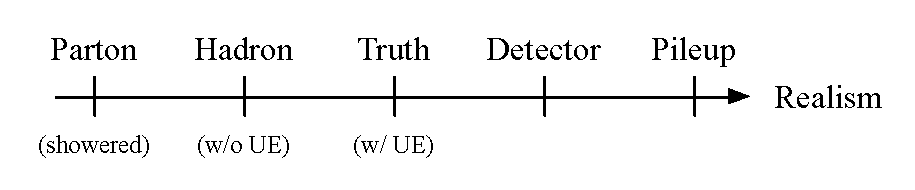
\includegraphics[width=0.75\columnwidth]{figures/realism_levels}
\end{center}
\caption{Realism}
\end{figure}


\begin{figure}
\begin{center}
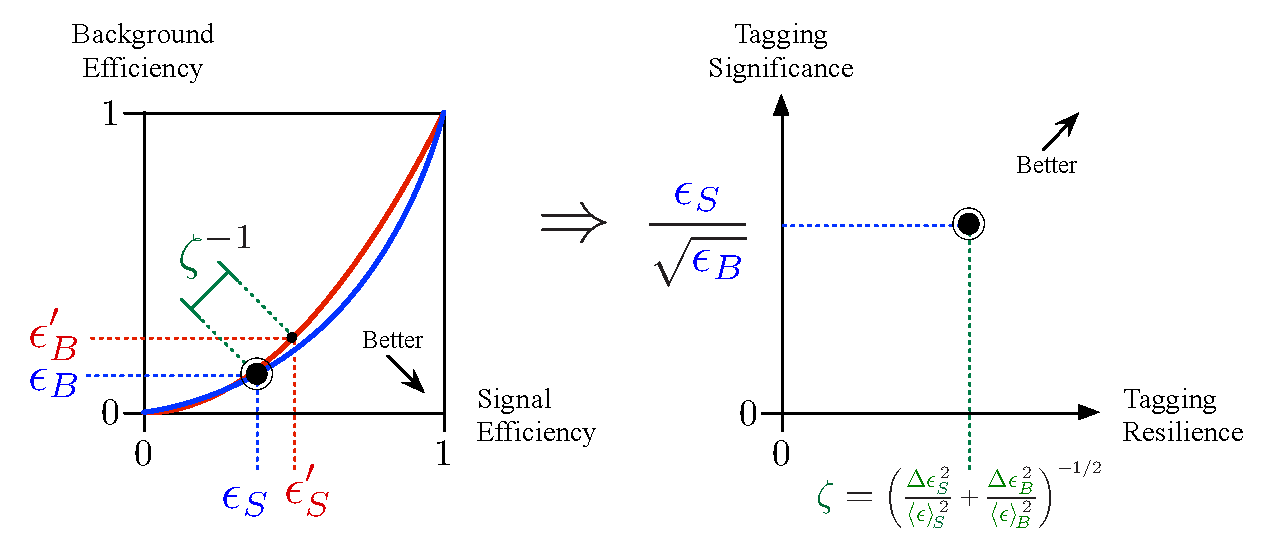
\includegraphics[width=1.0\columnwidth]{figures/roc_to_significance}
\end{center}
\caption{ROC to Significance}
\end{figure}

\ijm{explain the presentation of the results, and the metrics that we will use for quantifying the robustness}



\ijm{explain the different robustnesses that we will address, how they fit into the bigger 3d space.
Theory: hadronization, UE. Signal. Experiment}



%%%%%%%%%%%%%%%%%%%%%%%%%%%%%%%%%%%%%%%
\section{Observable Definitions}
%%%%%%%%%%%%%%%%%%%%%%%%%%%%%%%%%%%%%%%

In this section we summarize all the observable definitions and tagging approaches that will be studied throughout this paper. This includes the definition of the jet substructure shape observable, the definition of the grooming procedure, and the definition of the pile-up subtraction scheme. In \Sec{sec:hybrid_ratio} we will generalize the definitions of the ratio observables to allow for different levels of grooming in the numerator and the denominator.



%%%%%%%%%%%%%%%%%%%%%%%%%%%%%%%%%%%%%%%
\subsection{Jet Shape Observables}
%%%%%%%%%%%%%%%%%%%%%%%%%%%%%%%%%%%%%%%





\cite{Moult:2016cvt}

\begin{align}
\ecf{2}{\beta} &= \frac{1}{p_{TJ}^2}\sum_{1\leq i<j\leq n_J} p_{Ti}p_{Tj} R_{ij}^\beta \ ,\nonumber \\
\ecf{3}{\beta} &= \frac{1}{p_{TJ}^3}\sum_{1\leq i<j<k\leq n_J} p_{Ti}p_{Tj}p_{Tk} R_{ij}^\beta R_{ik}^\beta R_{jk}^\beta \ , \nonumber \\
\end{align}


\begin{equation}\label{eq:ecf_gen}
\ecfvar{v}{n}{\beta} = \sum_{1 \leq i_1 < i_2 < \dots < i_n \leq n_J} z_{i_1} z_{i_2} \dots z_{i_n} \prod_{m = 1}^{v} \min^{(m)}_{s < t \in \{i_1, i_2 , \dots, i_n \}} \left\{ \theta_{st}^{\beta} \right\},
\end{equation}
where $\min^{(m)}$ denotes the $m$-th smallest element in the list.  For a jet consisting of fewer than $n$ particles, $\ecfvarnobeta{v}{n}$ is defined to be zero.  More explicitly, the three arguments of the generalized energy correlation functions are as follows.
\begin{itemize}
\item The subscript $n$, appearing to the right of the observable, denotes the number of particles to be correlated.  This plays the same role as the $n$ subscript for the standard $e_n$ energy correlators in \Eq{eq:ECFs}. 
\item The subscript $v$, appearing to the left of the observable, denotes the number of pairwise angles entering the product.  By definition, we take $v \leq \binom{n}{2}$, and the minimum then isolates the product of the $v$ smallest pairwise angles.
\item The angular exponent $\beta>0$ can be used to adjust the weighting of the pairwise angles, as in \Eq{eq:ECFs}.
\end{itemize}
For the special case of $v = \binom{n}{2}$, the generalized energy correlators reduce to the standard ones in \Eq{eq:ECFs}, with $\ecfvarnobeta{1}{2}\equiv\ecfnobeta{2}$, $\ecfvarnobeta{3}{3}\equiv\ecfnobeta{3}$, $\ecfvarnobeta{6}{4}\equiv\ecfnobeta{4}$, and so on for the higher-point correlators. 

Compared to the original energy correlators, the generalization in \Eq{eq:ecf_gen} allows more flexibility in the angular scaling; this simplifies the construction of useful ratios and extends the possible applications of energy correlators.  In the case of boosted top tagging, for example, the standard $\ecfnobeta{4}=\ecfvarnobeta{6}{4}$ observable involves six different pairwise angles.  A decaying boosted top quark, however, does not have six characteristic angular scales, so most of these angles are redundant and only serve to complicate the structure of the observable.  This is reflected in the definition of $\Dobsnobeta{3}$ in \Eq{eq:D3_full_def}, which involves three distinct terms \cite{Larkoski:2014zma}.

To make more explicit the definition in \Eq{eq:ecf_gen}, we summarize the particular correlators used in our case studies below.  For boosted 2-prong tagging in \Sec{sec:2prong}, we use the 2-point energy correlation function
\begin{align}\label{eq:explicit_twopointvar}
\ecfvar{1}{2}{\beta}&\equiv\ecf{2}{\beta}=\sum_{1\leq i<j\leq n_J} z_{i}z_{j} \, \theta_{ij}^\beta\ ,
\end{align}
whose definition is unique, since it only involves only a single pairwise angle.  We also need the 3-point correlators, which have three variants probing different angular structures:\footnote{For $\ecfvarnobeta{2}{3}$, note that $\min\{{a,b,c}\} \times \min^{(2)} \{a,b,c\} = \min\{ab,ac,bc\}$.}
\begin{align}\label{eq:explicit_ecfvar}
\ecfvar{1}{3}{\beta}&=\sum_{1\leq i<j<k\leq n_J} z_{i}z_{j}z_{k} \min \left\{ \theta_{ij}^\beta\,,  \theta_{ik}^\beta\,, \theta_{jk}^\beta  \right\} \ , \nonumber \\
\ecfvar{2}{3}{\beta}&=\sum_{1\leq i<j<k\leq n_J} z_{i}z_{j}z_{k} \min \left\{\theta_{ij}^\beta \theta_{ik}^\beta\,, \theta_{ij}^\beta  \theta_{jk}^\beta\,,     \theta_{ik}^\beta \theta_{jk}^\beta    \right\}  \ , \nonumber \\
\ecf{3}{\beta}\equiv\ecfvar{3}{3}{\beta}&=\sum_{1\leq i<j<k\leq n_J} z_{i}z_{j}z_{k} \, \theta_{ij}^\beta \theta_{ik}^\beta \theta_{jk}^\beta \,.
\end{align}
Interestingly, we are able to construct powerful observables from each of these three 3-point correlators, resulting in different tagging properties.


\cite{Thaler:2011gf}\cite{Thaler:2010tr}

\begin{equation}\label{eq:nsubdef}
\Nsub{N}{\beta} = \frac{1}{p_{TJ}}\sum_{1\leq i \leq n_J} p_{Ti}\min\left\{
R_{i1}^\beta,\dotsc,R_{iN}^\beta
\right\} \ .
\end{equation}

$$
\Nsub{2,1}{\beta}\equiv \frac{\Nsub{2}{\beta}}{\Nsub{1}{\beta}} \quad\text{and}\quad \Nsub{3,2}{\beta}\equiv \frac{\Nsub{3}{\beta}}{\Nsub{2}{\beta}} \ ,
$$


It is convenient to work with dimensionless observables, written in terms of a generic energy fraction variable, $z$, and a generic angular variable, $\theta$. The precise definitions of the energy fraction and angle can be chosen depending on context and do not affect our power-counting arguments. For the case of $pp$ collisions at the LHC, which is the focus of our later studies, we work with longitudinally boost-invariant variables,
\begin{align}\label{eq:ptratio}  
z_i\equiv\frac{p_{Ti}}{\sum_{j \in \text{jet}} p_{Tj}}\,, \qquad  \theta_{ij}^2\equiv R_{ij}^2 = (\phi_i-\phi_j)^2+(y_i-y_j)^2\,,
\end{align}
where $p_{Ti}$, $\phi_i$, and $y_i$ are the transverse momentum, azimuthal angle, and rapidity of particle $i$, respectively. 
Two other measures intended for $e^+e^-$ collisions are available in the \texttt{EnergyCorrelator} \fastjet{contrib} \cite{Cacciari:2011ma,fjcontrib}.  The first is a definition based strictly on energies and opening angles,
\begin{align}\label{eq:Eratio}
z_i\equiv\frac{E_{i}}{E_{J}}\,,  \qquad \theta_{ij}^2\equiv \Theta_{ij}^2 \,,
\end{align}
where $E_J$ is the total jet energy, and $\Theta_{ij}$ is the Euclidean angle between the 3-momenta $\vec p_i$ and $\vec p_j$.  There is an alternative definition in terms of energies and Mandelstam invariants,
\begin{align}\label{eq:mandelstamratio}
z_i\equiv\frac{E_{i}}{E_{J}}\,,  \qquad \theta_{ij}^2\equiv\frac{2p_i \cdot p_j}{E_i E_j}  \,,
\end{align}
which reduces to \Eq{eq:Eratio} in the collinear limit but is easier for analytic calculations.

From \Eq{eq:ECFs}, we see that the $n$-point energy correlation functions vanish in the soft and collinear limits, and therefore are natural resolution variables for $(n-1)$-prong substructure.  A number of powerful 2-prong discriminants have been formed from the energy correlation functions  \cite{Larkoski:2013eya,Larkoski:2014gra}, namely
\begin{align}
\Cobs{2}{\beta}=\frac{\ecf{3}{\beta}}{(\ecf{2}{\beta})^{2}}\,,\qquad \Dobs{2}{\beta}=\frac{\ecf{3}{\beta}}{(\ecf{2}{\beta})^{3}}\,, \qquad \Dobs{2}{\alpha,\beta}=\frac{\ecf{3}{\alpha}}{(\ecf{2}{\beta})^{3\alpha/\beta}}\,.
\end{align}
Beyond their discrimination power, these observables have nice analytic properties.  First, since they can be written as a sum over particles in the jet without reference to external axes, they are automatically ``recoil-free'' \cite{Catani:1992jc,Dokshitzer:1998kz,Banfi:2004yd,Larkoski:2013eya,Larkoski:2014uqa}. Second, since they have well-defined behavior in various soft and collinear limits, they are amenable to resummed calculations;  in \Ref{Larkoski:2015kga}, $\Dobsnobeta{2}$ was calculated to next-to-leading-logarithmic (NLL) accuracy in $e^+e^-$ for both signal (boosted $Z$) and background (QCD) jets. 

\begin{equation}
N_i^{(\beta)} = \frac{\ecfvar{2}{i+1}{\beta}}{(\ecfvar{1}{i}{\beta})^2}\,,
\end{equation}

\cite{Moult:2016cvt}


\ijm{We want to consider}

\begin{itemize}
\item $N_2$
\item $D_2$
\item $\tau_{21}$
\end{itemize}

with $\beta=1,2$, and we will do it in the different dichroic forms.

%%%%%%%%%%%%%%%%%%%%%%%%%%%%%%%%%%%%%%%
\subsection{Grooming Techniques}
%%%%%%%%%%%%%%%%%%%%%%%%%%%%%%%%%%%%%%%

\ijm{need to generalize definitions to general beta}

Starting from a jet identified with an IRC safe jet algorithm (such as anti-$k_t$ \cite{Cacciari:2008gp}), the soft drop algorithm is defined using Cambridge/Aachen (C/A) reclustering \cite{Dokshitzer:1997in,Wobisch:1998wt,Wobisch:2000dk}.  Specializing to the case of $\beta=0$, the algorithm proceeds as follows:
\begin{enumerate}

\item Recluster the jet using the C/A clustering algorithm, producing an angular-ordered branching history for the jet.

\item Step through the branching history of the reclustered jet.  At each step, check the soft drop condition
\begin{align}\label{eq:sd_cut}
\frac{\min\left[ p_{Ti}, p_{Tj}  \right]}{p_{Ti}+p_{Tj}}> \zcut \,.
\end{align}
Here, $\zcut$ is a parameter defining the scale below which soft radiation is removed.  If the soft drop condition is not satisfied, then the softer of the two branches is removed from the jet.  This process is then iterated on the harder branch.

\item The soft drop procedure terminates once the soft drop condition is satisfied.

\end{enumerate}
Given a jet that has been groomed with the soft drop procedure, we can then measure any IRC safe observable on this jet and it will remain IRC safe.  


For the case that $\beta=0$, Soft Drop is equivalent to Modified Mass Drop \cite{Dasgupta:2013ihk}

\ijm{we will use }

loose: $\zcut=0.05$, $\beta=2$

tight: $\zcut=0.1$, $\beta=0$

trim: $R_{\text{sub}}=0.2$, fraction $0.05$



%%%%%%%%%%%%%%%%%%%%%%%%%%%%%%%%%%%%%%%
\subsection{Pile-Up Removal}
%%%%%%%%%%%%%%%%%%%%%%%%%%%%%%%%%%%%%%%

\ijm{Do this just at the level of the  detector simulation}

Area Subtraction\cite{Cacciari:2007fd}\cite{Cacciari:2008gn}

SoftKiller \cite{Cacciari:2014gra}

\begin{align}
\rho= \text{median} \left \{ \frac{p_{Ti}}{A_i}   \right \}
\end{align}

\begin{align}
p_t^{\text{cut}}=\text{median} \{ p_{Ti}^{\text{max}} \}
\end{align}

A variety of other approaches exist \cite{Bertolini:2014bba}\cite{Krohn:2013lba}   We take the above as representative.


%%%%%%%%%%%%%%%%%%%%%%%%%%%%%%%%%%%%%%%
\section{Theory Approaches to Robust Ratio Observables}\label{sec:hybrid_ratio}
%%%%%%%%%%%%%%%%%%%%%%%%%%%%%%%%%%%%%%%

\ijm{we need to define here how to extend the N, D, to dichroic variants}


\ijm{general interplay between more radiation (color flow), grooming which removes radiation, but improves robustness (both to np, and to pileup). Attempts to construct ratio observables that use mixes of groomed and ungroomed, and with different grooming amounts. How this is done for each of the different N2, D2 and tau21. Include some pictures of what this is doing. }

dichroic ratios:\cite{Salam:2016yht}

We will use the notation
\begin{align}
m \otimes \frac{n}{d}
\end{align}

In this form, $d$ is a mass type variable, and $n$ is a $3$ emision type variable. We want to have
\begin{align}
m \leq d \leq n
\end{align}

The division between $d$ and $n$

%%%
\begin{table}
\begin{center}
\begin{tabular}{| l | c | c |c |c|c|c |c|r| }
  \hline                       
  Observable &  Numerator & Denominator \\
  $N_2$ &   $\ecfvarnobeta{2}{3} / \ecfnobeta{2} $ & $ \ecfnobeta{2}$ \\
  $D_2$ &   $\ecfnobeta{3} / \ecfnobeta{2}^2 $ & $ \ecfnobeta{2}$ \\
  $\tau_{21}$ &   $\tau_2$ & $\tau_1$ \\
  \hline  
\end{tabular}
\end{center}
\caption{
denominator and numerator definition
}
\label{tab:PC}
\end{table}



%%%
\begin{table}
\begin{center}
\begin{tabular}{| l | c | c |c |c|c|c |c|r| }
  \hline                       
  Notation: $m \otimes \frac{n}{d}$ & Mass & Numerator & Denominator \\
  $p \otimes \frac{p}{p}$ & plain  &  plain & plain \\
  $l \otimes \frac{p}{p}$ & loose  &  plain & plain \\
  $l \otimes \frac{l}{p}$ & loose  &  loose & plain \\
  $t \otimes \frac{p}{p}$ & tight  &  plain & plain \\
  $t \otimes \frac{l}{p}$ & tight  &  loose & plain \\
  $t \otimes \frac{l}{l}$ & tight  &  loose & loose \\
  $t \otimes \frac{t}{p}$ & tight  &  tight & plain \\
  $t \otimes \frac{t}{l}$ & tight  &  tight & loose \\
  $t \otimes \frac{t}{t}$ & tight  &  tight & tight \\
  $trim$ & trim &  trim & trim \\
  \hline  
\end{tabular}
\end{center}
\caption{
Different observable combinations and notation
}
\label{tab:PC}
\end{table}

We will have plain, loose and tight grooming. 

We then have a variety of other options for how we combine the ratios


Representative of these different schemes are what is currently being used by CMS and ATLAS






%%%%%%%%%%%%%%%%%%%%%%%%%%%%%%%%%%%%%%%
\section{Samples and Detector Models}
%%%%%%%%%%%%%%%%%%%%%%%%%%%%%%%%%%%%%%%


%%%%%%%%%%%%%%%%%%%%%%%%%%%%%%%%%%%%%%%
\subsection{Samples}
%%%%%%%%%%%%%%%%%%%%%%%%%%%%%%%%%%%%%%%

Regarding the polarised $W$ samples, we consider a $gg$ produced resonance, $X$, that decays to a pair of polarized $W$ bosons. This kind of resonances decaying to longitudinally polarised $W$s appear in warped extra-dimensional models, where the SM fields propagate in the bulk. On the other hand, models with graviton-like tensor with minimal couplings yields only transversely polarized $W$ bosons. They were produced with the \textsc{JHUGEN} 3.1.8~\cite{Gao:2010qx,Bolognesi:2012mm} generator, interfaced with \textsc{PYTHIA} 8\cite{Sjostrand:2007gs} for parton showering including the effect of hard gluon radiation. Additional samples interfaced with \textsc{Herwig} 7~\cite{Bahr:2008pv,Bellm:2015jjp} were also used to study shower differences. A resonance width of 1\% was chosen. Table~\ref{table:polarisedSamples} shows the coupling values used to generate the polarised $W$ samples (see also Ref.~\cite{Gao:2010qx} for more information). 

\begin{table}[ht]
\caption{}
\centering
\begin{tabular}{c c c c}
\hline\hline
Model	&Production couplings	&Decay couplings	&Decay helicity amplitudes 	\\
\hline
$2_b^+$	& $g_1=1$		& $g_5=1$		& $f_{00}=0.98$			\\
$2_m^+$	& $g_1=1$		& $g_1=g_5=1$		& $f_{00}=0.08,f_{+-}=f_{-+}=0.46$\\	
\hline
\end{tabular}
\label{table:polarisedSamples}
\end{table}

Herwig Pythia hadronized, unhadronized, underlying event, WW, dijets

Herwig Pythia hadronized, unhadronized, underlying event, WW, dijets


%%%%%%%%%%%%%%%%%%%%%%%%%%%%%%%%%%%%%%%
\subsection{Detector Models}
%%%%%%%%%%%%%%%%%%%%%%%%%%%%%%%%%%%%%%%

\ijm{Description of TowerGrid}


%%%%%%%%%%%%%%%%%%%%%%%%%%%%%%%%%%%%%%%
\subsection{Summary of Parameters Scanned}
%%%%%%%%%%%%%%%%%%%%%%%%%%%%%%%%%%%%%%%

\ijm{Use $R$ as parameters}

$R=0.6,0.8,1.0,1.2$

$\beta=1,2$

substructure observables and different grooming combinations

$p_T=500,1000,2000$ GeV

%%%%%%%%%%%%%%%%%%%%%%%%%%%%%%%%%%%%%%%
\section{Signal Robustness (polarization)}
%%%%%%%%%%%%%%%%%%%%%%%%%%%%%%%%%%%%%%%

In this section we address two main issues, namely the robustness of the standard jet substructure observables to the polarization of the signals, and the ability to tag polarizations using jet substructure observables measured on the hadronic decay products.

%%%%%%%%%%%%%%%%%%%%%%%%%%%%%%%%%%%%%%%
\subsection{Robustness to Polarization}
%%%%%%%%%%%%%%%%%%%%%%%%%%%%%%%%%%%%%%%

%%%%%%%%%%%%%%%%%%%%%%%%%%%%%%%%%%%%%%%
\subsection{Tagging Polarization}
%%%%%%%%%%%%%%%%%%%%%%%%%%%%%%%%%%%%%%%

Having understood the robustness of the standard jet substructure observables to polarization, it is an interesting question to understand if jet substructure observables are able to separate distinct polarizations. Since the standard two prong tagging observables are not particularly sensitive to the polarization, a different observable must be used to tag polarizations. In this section we do not perform a comprehensive study, but restrict ourselves to studying a particular example of an observable which is sensitive to the $W$ polarization, and evaluate its performance for distinguishing transverse and longitudinal $W$ bosons. 

$z_g$\cite{Larkoski:2014wba}
\cite{Larkoski:2015lea}
\cite{Larkoski:2014bia}

%%%%%%%%%%%%%%%%%%%%%%%%%%%%%%%%%%%%%%%
\section{Theory Robustness (NP)}
%%%%%%%%%%%%%%%%%%%%%%%%%%%%%%%%%%%%%%%

\cite{Salam:2016yht}




We focus on hadronization and underlying event as main sources of theory uncertainty. These are not describable from first order calculations, and therefore it is desirable to minimize their impact in determining both the performance and distributions for substructure observables, if we want to have analytic calculations.

What is robustness?  (we will consider both ROC curve and effect on the distribution)

%%%%%%%%%%%%%%%%%%%%%%%%%%%%%%%%%%%%%%%
\subsection{Hadronization}
%%%%%%%%%%%%%%%%%%%%%%%%%%%%%%%%%%%%%%%

\ijm{compare between Pythia and Herwig based on different hadronization models}

effect of hadronization effects on two prong substructure observables has been studied in \cite{Larkoski:2015kga}\cite{Salam:2016yht}

shape functions: \cite{Korchemsky:1999kt,Korchemsky:2000kp,Bosch:2004th,Hoang:2007vb,Ligeti:2008ac}. Shape functions have support over a region of size $\Lambda_{\text{QCD}}$, and are convolved with the perturbative soft function. In the tail region of the distribution, where the observable is dominated by perturbative emissions, they reduce to a shift.  For a large class of observables, this shift is determined by a universal \cite{Akhoury:1995sp,Dokshitzer:1995zt} non-perturbative parameter multiplied by a calculable, observable dependent number \cite{Dokshitzer:1995zt,Lee:2006fn,Lee:2007jr}. 



%%%%%%%%%%%%%%%%%%%%%%%%%%%%%%%%%%%%%%%
\subsection{Underlying Event}
%%%%%%%%%%%%%%%%%%%%%%%%%%%%%%%%%%%%%%%

underlying event is less theoretically well understood, and less well defined. Here we take as a definition of underlying event what is generated in Pythia/Herwig

attempts to include with shape function \cite{Stewart:2014nna}


%%%%%%%%%%%%%%%%%%%%%%%%%%%%%%%%%%%%%%%
\section{Experimental Robustness (Detector)}
%%%%%%%%%%%%%%%%%%%%%%%%%%%%%%%%%%%%%%%


%%%%%%%%%%%%%%%%%%%%%%%%%%%%%%%%%%%%%%%
\subsection{TowerGrid Parameters}
%%%%%%%%%%%%%%%%%%%%%%%%%%%%%%%%%%%%%%%


%%%%%%%%%%%%%%%%%%%%%%%%%%%%%%%%%%%%%%%
\subsection{Very high pT (detector)}
%%%%%%%%%%%%%%%%%%%%%%%%%%%%%%%%%%%%%%%


%\section{Jet Radius Robustness:  High pT (isolation versus shape cut, jet radius)}

%\ijm{I think no longer have this in this separate section}




%%%%%%%%%%%%%%%%%%%%%%%%%%%%%%%%%%%%%
\section{Understanding ATLAS vs. CMS}
%%%%%%%%%%%%%%%%%%%%%%%%%%%%%%%%%%%%%

\ijm{The strategies used by ATLAS and CMS are representative of the schemes above. }

D2:\cite{Larkoski:2015kga}\cite{Larkoski:2014gra}

N2:\cite{Moult:2016cvt}
with DDT:\cite{Dolen:2016kst}

\ijm{I think for our purposes we can ignore the DDT. }

%%%%%%%%%%%%%%%%%%%%%%%%%%%%%%%%%%%%%%%
\section{Conclusions}
%%%%%%%%%%%%%%%%%%%%%%%%%%%%%%%%%%%%%%%

In this paper, we have

similar approaches could also be applied to study $3$-prong tagging...


%%%%%%%%%%%%%%%%%%%%%%%%%%%%%%%%%%%%%%%
\begin{acknowledgments}
%%%%%%%%%%%%%%%%%%%%%%%%%%%%%%%%%%%%%%%


The work of GS is supported in part by the Paris-Saclay IDEX under the
IDEOPTIMALJE grant, by the French Agence Nationale de la Recherche,
under grant ANR-15-CE31-0016, and by the ERC Advanced Grant Higgs@LHC
(No.\ 321133).
%
The work of JT is supported by the DOE under grant contract numbers DE-SC-00012567 and DE-SC-00015476.


%%%%%%%%%%%%%%%%%%%%%%%%%%%%%%%%%%%%%%%
\end{acknowledgments}
%%%%%%%%%%%%%%%%%%%%%%%%%%%%%%%%%%%%%%%



\appendix

%\section{Introduction}
%\label{sec:introduction}
%
%Variety of 2-prong taggers, want to understand behavior.  Focus on W bosons.  No b-tagging.  
%
%(3-prong is future)
%
%new physics robustness?
%
%Goals:  understand ATLAS/CMS differences (summary section, it is a byproduct of detector sensitivity, or of truth-level), very high pT behavior,  interplay of jet radius, jet grooming, jet discrimination.  Groomed/ungroomed/dichroic observables.  Detector effects (simplified)
%
%(polarization is separate study?  Or initial study?)
%
%Also interesting in tagging longitudinal vs. transverse W bosons

%\subsection{Brainstorm}
%
%Three dimensional space:  efficiency (performance), NP robustness, detector robustness
%
%1)  Theory-level projection:  efficiency (performance), NP robustness,
%
%both for fixed and variable cuts
%
%we should be able to understand sensitivity (on theory land)
%
%split hadronization and underlying
%
%2)  Experiment:  efficiency vs. detector robustness
%
%
%1) Difference between modern tools on groomed versus ungroomed at truth level  (motivation
%
%2) How affected by pileup/detector effects


%\section{Preliminaries}
%
%\subsection{Event Samples}
%
%WW Pythia 8 pTW > 500 GeV
%
%Need polarized Ws
%
%Need dijet samples
%
%Pileup Samples from pileup study
%
%\subsection{Observables}
%
%CMS:  mMDT mass, ungroomed N2
%ATLAS:  trimmed mass, trimmed D2
%
%\subsection{Detector Simulation}
%
%Do we do DELPHES?
%
%TowerGrid from Peter, included ATLAS/CMS B-field
%
%Calorimetry vs. Particle Flow

%\section{Particle-Level Tagging}
%
%\subsection{Unpolarized Case}
%
%\subsection{Longitudinal versus Transverse Polarization}
%
%\subsection{Adjusting the Jet Radius}
%
%\section{Impact of Detector Effects}
%
%\subsection{Mass Resolution}
%
%\subsection{Tagging Performance}
%
%\subsection{Behavior in the Ultra-boosted Regime}
%
%\section{Comparison of ATLAS and CMS Two-prong Strategies}
%
%
%\section{Conclusions}



\bibliographystyle{jhep}
\bibliography{lh2017_2prong}

\end{document}
